\documentclass[12pt,oneside]{article}
\usepackage{light}
\usepackage{multicol}
\usepackage{pifont} % for the star
\usepackage{palatino}
\usepackage{mathpazo}
\usepackage{verbatim}

\newcommand{\mfigure}[3]{\bigskip\centerline{\resizebox{#1}{#2}{\includegraphics{#3}}}\bigskip}
\newcommand{\hint}[1]{({\it Hint: #1})}
\newcommand{\brule}[1]{\underline{\hspace{#1}}}
\newcommand{\ang}[1]{\left< #1 \right>}
\newcommand{\beats}{\rightarrow}


\newenvironment{falseproof}
{\begin{proof}[False proof]}
{\end{proof}}

%\showsolutions
\hidesolutions

\begin{document}
\generic{Final}{December 14, 2010}

\instatements{
\vspace{12pt}
\textbf{Name:} \rule{5in}{0.5pt}

\textbf{Circle the name of your recitation instructor}:

\begin{center}
\begin{tabular}{llllll}
David & Darren & Martyna & Nick & Oscar & Stav 
\end{tabular}
\end{center}

\begin{itemize}

\item This quiz is \textbf{closed book}, but you may have one $8.5
\times 11$'' sheet with notes in your own handwriting on both sides.

\item Calculators are not allowed.

\item You may assume all of the results presented in class.

\item Please show your work.  Partial credit cannot be given for a wrong
answer if your work isn't shown.

\item Write your solutions in the space provided.  If you
need more space, write on the back of the sheet containing the
problem.  Please keep your entire answer to a problem on that
problem's page.

\item Be neat and write legibly.  You will be graded not only on the
correctness of your answers, but also on the clarity with which you
express them.

\item If you get stuck on a problem, move on to others. The problems 
are not arranged in order of difficulty.

\item The exam ends at 4:30 PM.

\end{itemize}

\vspace{0.25in}

\begin{center}
{\large
\begin{tabular}{|c|c|c|c|}
\hline
Problem & Points & Grade & Grader \\ \hline \hline
1 & 10 & & \\ \hline
2 & 10 & & \\ \hline
3 & 20 & & \\ \hline
4 & 15 & & \\ \hline
5 & 20 & & \\ \hline
6 & 25 & & \\ \hline
7 & 10 & & \\ \hline
8 & 10 & & \\ \hline
Total & 120 & & \\ \hline
\end{tabular}
}
\end{center}
}
\instatements{\newpage}


%%%%%%%%%%%%%%%%%%%%%%%%%%%%%%%%%%%%%%%%%%%%%%%%%%%%%%%%%%%%%%%%%%%%%%%%%%%%%%%%%%%%%%%%%%%%%%%%%%%%%%%%%%%%%%%%%%%%%%%%%%%%%%%%%%%%%%%%%%%%%
% PROBLEM 1

\begin{problem}{10}

Consider the recursion 

$$T_{n+2} = T_{n+1} + 2T_{n}, T_0 = T_1 = 1$$

\bparts
	\ppart{5} Show that $T_n$ is odd
	
	\vspace{4 in}
	
	\ppart{5} Using part (a), prove that $\gcd(T_{n+1}, T_{n}) = 1$.  Note that
	this implies that $T_{n+1}$ and $T_n$ are relatively prime.
\eparts

\solution{
solution
}
\end{problem}

\newpage

%%%%%%%%%%%%%%%%%%%%%%%%%%%%%%%%%%%%%%%%%%%%%%%%%%%%%%%%%%%%%%%%%%%%%%%%%%%%%%%%%%%%%%%%%%%%%%%%%%%%%%%%%%%%%%%%%%%%%%%%%%%%%%%%%%%%%%%%%%%%%
% PROBLEM 2
\begin{problem}{10}
Let $R$ be a positive random variable with $E[R^3] = k$. Show $Pr(R \geq x) \leq k/x^3$
\end{problem}

%
%\begin{problem}{10}
%In this problem we explore a variation of the famous Monty Hall Problem. The set up will be as follows:
%
%Suppose you are on a game show, and are given the choice of three doors, A, B, and C. Behind one door is a car and behind the other two doors are goats. The car is equally likely to be hidden behind each of the three doors. You pick a door. If you have selected the door that hides the car, the host will open one of the remaining doors (with equal probability) and offer you to switch doors. This is just as in the original Monty Hall problem.
%
%Otherwise, if you pick a door without the car, the host will do one of two things:
%\begin{enumerate}
%\item With probability 0.5 the host will immediately open the door that you have selected, revealing a goat. In this case you will always lose.
%\item With probability 0.5 he will open the other door that does not contain the car. The host will then give you the opportunity to switch doors.
%\end{enumerate}
%
%After this is completed, the door you selected is opened. If that car is hidden behind it, you win a car! Otherwise you lose.
%\bparts
%\ppart{5}
%What is the probability of winning the car if initially you select door 3 and you always switch if you are offered the opportunity to switch?
%
%\newpage
%\ppart{5}
%What is the probability of winning the car if initially you select door 3 and if the host opens door 2 you switch otherwise you stick with door 3?
%
%\eparts
%\end{problem}
%
%
%\newpage


%%%%%%%%%%%%%%%%%%%%%%%%%%%%%%%%%%%%%%%%%%%%%%%%%%%%%%%%%%%%%%%%%%%%%%%%%%%%%%%%%%%%%%%%%%%%%%%%%%%%%%%%%%%%%%%%%%%%%%%%%%%%%%%%%%%%%%%%%%%%%
% PROBLEM 3

%\begin{problem}{20}
%
%\bparts
%\ppart{5}
%An $n \times m$ chessboard (a board with squares colored black and white) can be covered with T-shaped tetris blocks like the ones in the figure below. Prove that the number of black squares on that chessboard must be even.
%\hint{What can sizes can the chessboard have?}
%\begin{center}
%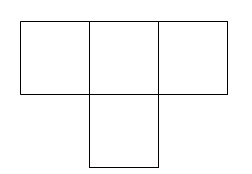
\includegraphics{tetris.jpg}
%\end{center}
%\begin{center}
%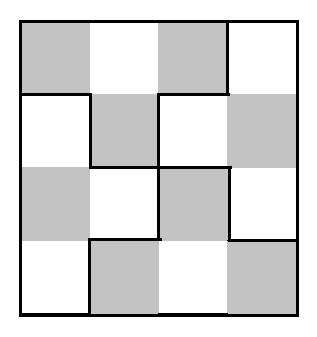
\includegraphics{chessboard.jpg}
%\end{center}
%\solution{Number of squares divisible by $4$. Two cases: both sides even length or one side with length divisible by $4$.}
%
%\newpage
%\ppart{15}
%Prove that the number of squares on the chessboard is divisible by $8$.
%\hint{Use part a and think about what color squares one T-shaped tetris block covers.}
%\solution{(Sketch) Each block covers $3$ black and $1$ white or $1$ black and $3$ white squares. Show by induction that an odd number of blocks covers an odd number of black squares. Number of black squares is even, so need an even number of blocks. Each of them is of size $4$, so they cover a multiple of $8$ squares.}
%\eparts
%\end{problem}
%\newpage
%%%%%%%%%%%%%%%%%%%%%%%%%%%%%%%%%%%%%%%%%%%%%%%%%%%%%%%%%%%%%%%%%%%%%%%%%%%%%%%%%%%%%%%%%%%%%%%%%%%%%%%%%%%%%%%%%%%%%%%%%%%%%%%%%%%%%%%%%%%%%
% PROBLEM 4


\begin{problem}{20}
In the far off land of Spain two soccer teams: Barcelona and Madrid have been battling each other for centuries to see who is more awesome. They play two games a year: one in the Spring and one in the Fall. The Madrid team has a tendency to fire their coaches very often to try to improve their results. The outcomes of the games are as follows:
\begin{enumerate}
\item
If Madrid has not just fired their coach:
\begin{itemize}
\item
Barcelona wins with probability $\frac25$
\item
Madrid wins with probability $\frac25$
\item
They tie with probability $\frac15$
\end{itemize}
\item
If Madrid has just fired their coach (they haven't yet realized that it's a bad idea):
\begin{itemize}
\item
Barcelona wins with probability $\frac35$
\item
Madrid wins with probability $\frac15$
\item
They tie with probability $\frac15$
\end{itemize}
\end{enumerate}
Now, Madrid does not fire their coach if they win or tie, but if Barcelona wins, they will fire their coach with $90\%$ probability.
For the following two questions, assume that Madrid did not fire their coach before the Spring 2010 game.

\bparts
\ppart{10}
Given that Madrid lost the Fall 2010 game, what is the probability that they fired their coach between the Spring and Fall games this year.

\newpage
\ppart{10}
What is the probability that Madrid fired their coach between the Spring and Fall games this year given that they lost BOTH of these games?
\eparts
\end{problem}

\newpage
%%%%%%%%%%%%%%%%%%%%%%%%%%%%%%%%%%%%%%%%%%%%%%%%%%%%%%%%%%%%%%%%%%%%%%%%%%%%%%%%%%%%%%%%%%%%%%%%%%%%%%%%%%%%%%%%%%%%%%%%%%%%%%%%%%%%%%%%%%%%%
% PROBLEM 5

\begin{problem}{25}
\bparts
%\ppart{5}
%You repeatedly roll a fair die. What is the probability that you will roll a $5$ before you roll a $6$?
\ppart{5}
You roll two fair dice and look at the sum. What is the expected value of that sum? 
\vspace{4 in}

\ppart{5}
What is the variance?
\vspace{4 in}


\ppart{5}
You repeatedly roll two fair dice and look at the sum. What is the probability that you will roll a sum of $4$ before you roll a sum of $7$?
\vspace{4 in}

\ppart{5}
What is the expected number of rolls before you get a sum of $4$ or a sum of $7$?

%\vspace{4 in}
%
%\ppart{5}
%What is the probability that you will roll a sum of $4$ and a sum of $10$ before you roll a sum of $7$?

\vspace{4 in}

\ppart{5}
You roll 10 dice.  Using the Chernoff Bound, give an upper bound for the probability that 8 or more of them rolled a 1 or a 2?  

\vspace{4 in}

\ppart{5}
Recall that we can approximate the CDF of the binomial distribution by $F_{n,p}(\alpha)$
whenever $\alpha < p$.  In terms of $F_{n, p}(\alpha)$, give an upper bound for
the probability that 8 or more of them rolled a 1 or a 2?


\eparts
\end{problem}

\newpage

%%%%%%%%%%%%%%%%%%%%%%%%%%%%%%%%%%%%%%%%%%%%%%%%%%%%%%%%%%%%%%%%%%%%%%%%%%%%%%%%%%%%%%%%%%%%%%%%%%%%%%%%%%%%%%%%%%%%%%%%%%%%%%%%%%%%%%%%%%%%%
% PROBLEM 6
%
%\begin{problem}{20}
%In class, we have shown that the congestion of a butterfly network is $\sqrt{N}$. In this problem, we will analyze the expected number of packages going through a specific switch in the network. Recall that if you look at the switch in the $i-th$ layer of the network and represent it's position in that layer as a binary number $(y_1y_2\ldots y_ix_{i+1}x_{i+1}\ldots x_{n})$ where $N=2^n$, then the packets going through that switch are the ones where the output starts with $y_1y_2\ldots y_i$ in binary AND the input ends with $x_{i+1}x_{i+1}\ldots x_{n}$ in binary.
%Assume you are given a random assignment of outputs to inputs. How many packets do you expect to go through a switch in the $i-th$ layer of the network?
%\solution{
%Let $X_j$ be the indicator random variable that the packet from input $j$ goes through our switch and let $E_j$ be the indicator variable that $j$ ends with  $x_{i+1}x_{i+1}\ldots x_{n}$ in binary representation. We have two cases.
%\begin{enumerate}
%\item
%$Pr(X_j=0|E_j=0)=1$.
%\item
%$Pr(X_j=1|E_j=1)=\frac{1}{2^x}$ and $Pr(X_j=0|E_j=1) = 1-frac{1}{2^x}.
%\end{itemize}
%Therefore $Ex(X_j)=\frac{1}{2^x} \cdot E_j.
%Consequently,
%\begin{eqnarray*}
%Ex(number of packets through switch) &=& \sum_{j=0}^{N-1}Ex(X_j)\\
%& = &\sum_{j=0}^{N-1}\frac{1}{2^x} \cdot E_j\\
%& = &\frac{1}{2^x}\sum_{j=0}^{N-1}E_j\\
%& = &\frac{1}{2^x} \cdot (number of inputs that start with $x_{i+1}x_{i+1}\ldots x_{n}$ in binary representation)\\
%& = &\frac{1}{2^x} \cdot 2^x\\
%& = & 1.
%\end{eqnarray*}
%}
%\end{problem}


\newpage
%%%%%%%%%%%%%%%%%%%%%%%%%%%%%%%%%%%%%%%%%%%%%%%%%%%%%%%%%%%%%%%%%%%%%%%%%%%%%%%%%%%%%%%%%%%%%%%%%%%%%%%%%%%%%%%%%%%%%%%%%%%%%%%%%%%%%%%%%%%%%
% PROBLEM 7

\begin{problem}{15}
Show that for any $m,n,k$ such that $k<m<n-k$, the following identity holds:
\[ \binom{n}{k} = \sum_{i=0}^{k} {\binom{m}{i}} \cdot {\binom{n-m}{k-i}}\]
\solution{
Select $k$ people from a group of $n$ by splitting the people into two groups of $m$ and $n-m$, each with at least $k$ people, and then select $i$ from first group and $k-i$ from second group.
}
\end{problem}


\newpage
%%%%%%%%%%%%%%%%%%%%%%%%%%%%%%%%%%%%%%%%%%%%%%%%%%%%%%%%%%%%%%%%%%%%%%%%%%%%%%%%%%%%%%%%%%%%%%%%%%%%%%%%%%%%%%%%%%%%%%%%%%%%%%%%%%%%%%%%%%%%%
% PROBLEM 8

\begin{problem}{10}

\bparts
\ppart{5}
Three sets of twins are sharing a bucket of 24 pieces of chicken from Olive Oyl's.  If each person eats at least one piece of chicken, how many ways can the chicken pieces be distributed amongst this family?  You do not have to calculate a specific number, but please give your answer in a closed form (no summations).  Also,
for the purposes of this problem, chicken pieces are indistinguishable.

\vspace{3 in}

\ppart{5}

Across town, a family of seven folk eat a meal that comes with unlimited sides of biscuits (the restaurant owner has deep pockets).  Being a caring family, some number of biscuits are shared between the family members.  However, the family obeys the following two rules:

\begin{itemize}
	\item If a biscuit is shared, it must be shard between \textbf{exactly two} people
	\item If two people share a biscuit, they cannot share another biscuit.  
\end{itemize}

Prove that there exist two members of this family who shared the same number of biscuits as each other.
\vspace{4 in}

\eparts
\end{problem}


\newpage
%%%%%%%%%%%%%%%%%%%%%%%%%%%%%%%%%%%%%%%%%%%%%%%%%%%%%%%%%%%%%%%%%%%%%%%%%%%%%%%%%%%%%%%%%%%%%%%%%%%%%%%%%%%%%%%%%%%%%%%%%%%%%%%%%%%%%%%%%%%%%
% PROBLEM 9

\begin{problem}{10}

Find a closed-form solution to the following recurrence: 

$x_n = 11x_{n-1} - 30x_{n-2}$ where $(x_0 =4, x_1 = 23)$
\end{problem}

\newpage
%%%%%%%%%%%%%%%%%%%%%%%%%%%%%%%%%%%%%%%%%%%%%%%%%%%%%%%%%%%%%%%%%%%%%%%%%%%%%%%%%%%%%%%%%%%%%%%%%%%%%%%%%%%%%%%%%%%%%%%%%%%%%%%%%%%%%%%%%%%%%
% PROBLEM 10

\begin{problem}{20}
\bparts
\ppart{10}
Show that in any direct acyclic graph there exists a node with no outgoing edges.
\solution{By contradiction. Look at the longest path.}

\vspace{4 in}

\ppart{10}
Show that any direct acyclic graph with maximum in-degree $k$ is $k+1$-colorable.
\solution{Induction on number of nodes.}
\eparts
\end{problem}

\newpage
%%%%%%%%%%%%%%%%%%%%%%%%%%%%%%%%%%%%%%%%%%%%%%%%%%%%%%%%%%%%%%%%%%%%%%%%%%%%%%%%%%%%%%%%%%%%%%%%%%%%%%%%%%%%%%%%%%%%%%%%%%%%%%%%%%%%%%%%%%%%%
% PROBLEM 11

\begin{problem}{10}
Let G be a bipartite graph with $n$ nodes and $k$ components. You independently color each of the nodes of $G$ red or black with equal probabilities. What is the probability that your coloring is a valid $2$-coloring of $G$?
\solution
{There are $2$ ways to correctly color each component, and there are $k$ components, so there is $2^k$ valid colorings. The number of colorings you might produce is $2^n$ and each is equallly likely. The probability that you get a valid coloring is 
\[\frac{2^k}{2^n} = \frac{2^{k-n}}\]
}
\end{problem}


\newpage
%%%%%%%%%%%%%%%%%%%%%%%%%%%%%%%%%%%%%%%%%%%%%%%%%%%%%%%%%%%%%%%%%%%%%%%%%%%%%%%%%%%%%%%%%%%%%%%%%%%%%%%%%%%%%%%%%%%%%%%%%%%%%%%%%%%%%%%%%%%%%
% PROBLEM 12

\begin{problem} %%oscar, reformulated from 06 final. Will need to check wording. May modify solutions for clearer answer. 
{\bf [10 points]}
There is a complete deck of 52 cards, and half of another deck (for a total of 52 + 26 cards) left over. The decks have been mixed together, and repeated cards cannot be told apart. A hand of 5 cards is picked randoly from the shuffled deck and a half.


\ppart {\bf [5 points]} What is the probability that the hand has no identical cards (i.e., cards with the same suit and value. For example, the hand {$\left<Q\heartsuit, 5\spadesuit, 6\spadesuit, 8\clubsuit, Q\heartsuit\right>$} {\em has} identical cards.)?  (you can leave your answer in terms of binomial coefficients)
\vspace{.15in}

We can calculate this probability by calculating
%
\[
\frac{\text{hands with no identical cards}}{\text{total possible hands}}
\]
%

Note there are essentially two families of types (the type of a card is its (suit, number)  pair) of cards: 26 types are repeated in the set and 26 are unique in the set.  We can count the number of possible hands with no identical cards by considering the following cases: the hand is made out of 5 cards of non-repeated types, the hand is made out of 4 cards of non-repeated types in the set and 1 of a repeated type, ... up to the case of all cards are of repeated types. If all cards are from the non repeated kind, there are only $\binom{52}{5}$ possibilities. If all cards are from the repeated types, then we have $\binom{52}{5}\cdot2^5$ hands that could be created. If the hand has $k$ cards from the non-repeated types and $5 - k$ from the repeated types,  then there are $\binom{52}{k}\cdot \binom{52}{5-k} \cdot 2^{5 - k}$ possible hands.

So we get a total count of:

\[
\sum_{i = 0}^5 \binom{52}{k}\cdot \binom{52}{5-k} \cdot 2^{k-5}
\]


Therefore the probability of drawing a hand with no identical cards is:

%
\[
\frac{\sum_{i = 0}^5 \binom{52}{k}\cdot \binom{52}{5-k} \cdot 2^{k-5}}{\binom{78}{5}}
\]
%
\vspace{4 in}

\ppart {\bf [5 points]} What is the probability that the hand has exactly two pairs of identical cards?
\vspace{.15in}

If we have two pairs of identical cards, both pairs will be of the repeated kinds. All possible hands of this type can be concisely described by a tuple $\left( \{T_1, T_2\}, t \right)$ where $\{T_1, T_2\}$ is a set of the two distinct types that appear twice, and $t$ is any leftover card.  There are $\binom{26}{2}$ options for the set, and $52 + 26 - 4 = 74$ options for the third card.

Hence the probability we pick such a hand is:
%
\[
\frac{\binom{26}{2}\cdot 74}{\binom{78}{5}}
\]
%

%\eparts
\end{problem}

\newpage
%%%%%%%%%%%%%%%%%%%%%%%%%%%%%%%%%%%%%%%%%%%%%%%%%%%%%%%%%%%%%%%%%%%%%%%%%%%%%%%%%%%%%%%%%%%%%%%%%%%%%%%%%%%%%%%%%%%%%%%%%%%%%%%%%%%%%%%%%%%%%
% PROBLEM 13


\begin{problem}{10}

Consider a length $n$ vector of integers, $x = (x_1, x_2, \ldots, x_n)$ where the entries
of the vector are integers in the set $\{1, 2, \ldots, n \}$.  Let $A$ be the number of 
entries $x_i$ in the vector where $x_i \leq i$.  
\bparts
	\ppart{5}
		Calculate $E[A]$.
		
		\vspace{4 in}
		
	\ppart{5}
		Calculaate the variance of $A$.
		
		\vspace{4 in}
\eparts


\end{problem}

\newpage
\begin{problem}{20}
In the card game of bridge, you are dealt a hand of $13$ cards from the standard $52$-card deck.
\bparts

\ppart{5}
A balanced hand is one in which a player has roughly the same number of cards in each suit. How many different hands are there where the player has $4$ cards in one suit and $3$ cards in each of the other suits?
\solution{There are $4$ suits to pick from for the longest suit, $4$ cards out of $13$ to choose from in that suit, and $3$ cards out of $13$ to choose from in each of the remaining $3$ suits.
This gives
\[4\cdot\binom{13}4\cdot\binom{13}{3} \cdot\binom{13}{3}\cdot\binom{13}{3}\]
such hands.}
\vspace{4 in}

\ppart{5}
Not surprisingly, a non-balanced hand is one in which a player has more cards in some suits than others. Hands that are very disired are ones where over half the cards are in one suit. How many different hands are there where there is exactly $7$ cards in one suit?
\solution{
There are $4$ suits to choose from for the long suit, $7$ cards out of $13$ to choose in that suit, and $6$ cards out of the remaining $39$ in the other $3$ suits. This gives
\[4\cdot\binom{13}{7}\cdot\binom{39}6\]
such hands.
}
\eparts
\end{problem}


\newpage

\newpage
\begin{center}
(Notes)
\end{center}

\newpage

\mbox{}

\newpage

\mbox{}

\end{document}
